\section{Testing}
Um die Applikation auf Erfüllung der für ihren Einsatz definierten
Anforderungen zu bewerten und zu prüfen sind Softwaretests nötig. Es wurde
versucht, diese Tests am Anfang zu erstellen und im Laufe der Entwicklung
regelmässig zu durchführen und erweitern. Es wurden in der Regel zwei Arten
von Tests eingesetzt: manuelle und automatisierte Tests. Die manuellen Tests
wurden einerseits mit dem Debugger zur Verifizierung der Inhalte und
andererseits mit systematisch festgelegten Eingabedaten ausgeführt. Daneben
wurden auch noch die automatisierten Unit-Tests eingesetzt, um zu
verifizieren, dass bei Änderungen keine unerwünschten Nebeneffekte
auftreten. 

In unserer Appkilation wurden für alle Packages mindestens ein JUnit-Test
geschrieben. Entweder werden ganze Klassen oder nur gewisse, essenzielle
Methoden getestet. Somit sollten diese Tests die meisten Fällen abdecken. 

\subsection{JUnit Test}
JUnit ist ein kleines, mächtiges Java-Framework zum Schreiben und Ausführen
von automatisierten Unit-Tests. Es wird in der Regel für alle Klassen, die
überprüft werden sollen, ein Unit-Test erstellt. Diese Unit-Tests verhalten
sich auch wie die gewöhnlichen Java-Klassen, mit dem Unterschied, dass sie im
Namen das Wort \texttt{Test} am Schluss und einige JUnit-Annotationen innerhalb der
Klasse haben, wobei die Endung im Namen nur eine Konvention ist. Ein
JUnit-Test kennt nur zwei Ergebnisse: Entweder war der Test erfolgreich oder
nicht. Das Fehlschlagen kann zwei Gründe haben, entweder war es ein
Fehler (Error) oder es lieferte ein falsches Ergebnis (Failure). Der einzige
Unterschied zwischen den beiden Begriffen liegt darin, dass Errors eher
unerwartet auftreten, während Failures erwartet werden. Desweiteren können die
geschriebenen Testfälle zu jeder Zeit wiederholt werden. 

Ausserdem bietet dieses Framework einige Methoden an, um Werte vergleichen zu
können. So zum Beispiel vergleicht die Methode \texttt{assertEquals(expected, actual,
delta)} zwei Werte, expected und actual, und kann eine Abweichung
\texttt{delta} beinhalten. 

\subsubsection{Beispiele}
Als Beispiel für ein JUnit-Test kann der Test für die Klasse
\texttt{TrackComputation} gebracht werden. Diese Klasse berechnet den Winkel
zwischen zwei Punkten $A$ und $B$. Für die Berechnung wurden simple
Beispieldaten genommen, um das Resultat auch selbst nachvollziehen zu können.
Diese Daten wurden in einer \texttt{HashMap} gespeichert. Ein \texttt{HashMap}
ist ein Assoziativspeicher.  D.h. dass diese Klasse Datenelemente mit
Schlüssel und Wert-Paaren abspeichert. In unserem Beispiel fungiert sie eher
als eine Liste.  Danach werden diese Werte ausgelesen und der Winkel
berechnet. Falls die berechneten Winkel mit den \texttt{Mathematica} Lösungen
übereinstimmen, war der Test erfolgreich (grün).

Der JUnit-Test sieht wie folgt aus:

\lstinputlisting[label=src:trackComp,caption=JUnit-Test für die Klasse TrackComputation]{code/trackComputationTest.java}

Da der Windfeld-Container mehrere Windfelder hat, wurden auch einige Simulationen 
zur besseren Veranschaulichung und der Nachvollziehbarkeit durchgeführt. Es wurde versucht,
möglichst verschiedene Routen berechnen und zeichnen zu lassen, um die Korrektheit des
Algorithmus aufzuzeigen. 

Das erste Beispiel soll aufzeigen, wie die optimale Route einen Zick-Zack Kurs einnehmen muss,
um am schnellsten am Ziel anzukommen:

\begin{figure}[h!]
\centering
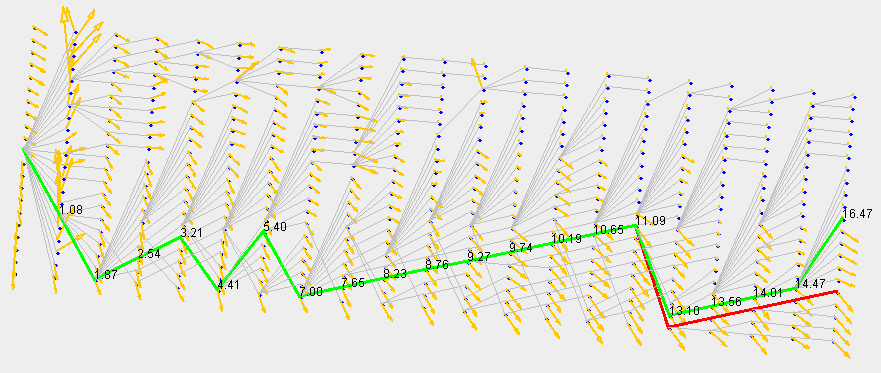
\includegraphics[width=0.8\linewidth]{img/gridNet_1}
\caption{Zick-Zack Kurs für die optimale Lösung.}
\label{gridnet1}
\end{figure}

Dieses Beispiel zeigt eine primitive und glatte Lösung, da die Windvektoren
schon einigermassen in diese Richtung zeigen:

\begin{figure}[h!]
\centering
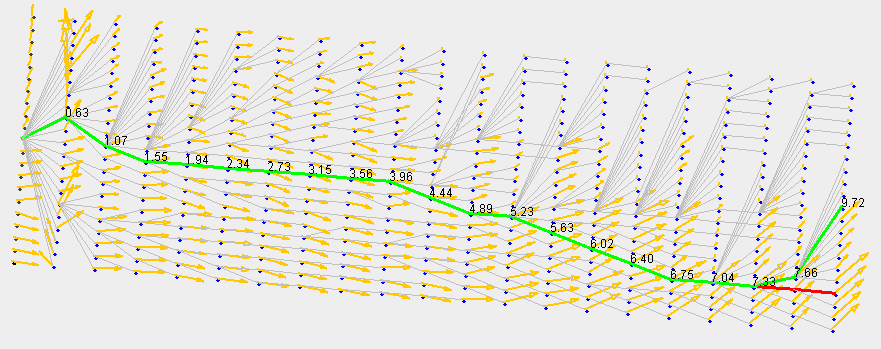
\includegraphics[width=0.8\linewidth]{img/gridNet_2}
\caption{Primitiver und glatter Kurs für die optimale Lösung.}
\label{gridnet2}
\end{figure}

Als letztes Veraunschaulicht dieses Beispiel eine Route, die ihren Kurs in der
Mitte ändern muss, da die Richtungen der Windvektoren sich gekehrt haben. 

\begin{figure}[h!]
\centering
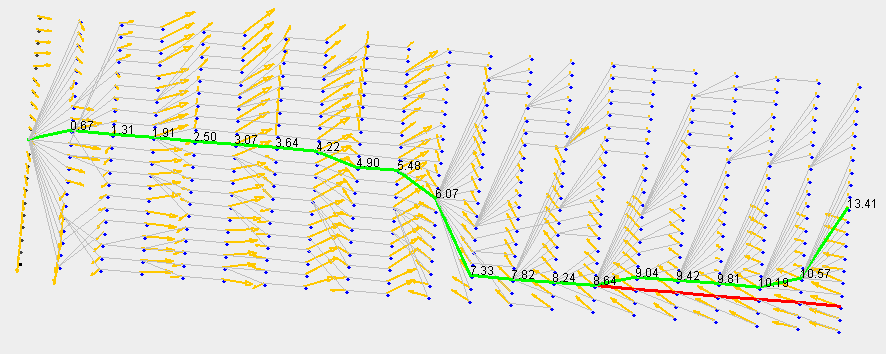
\includegraphics[width=0.8\linewidth]{img/gridNet_20}
\caption{Änderung des Kurses in der Mitte für die optimale Lösung.}
\label{gridnet3}
\end{figure}
